\documentclass[10pt]{article}

\usepackage[T1]{fontenc}
\usepackage{geometry}
\usepackage{amsmath, amssymb, amsthm}
\usepackage{yhmath}
\usepackage{graphicx}
\usepackage{xcolor}
\usepackage{float}
\usepackage{bm}
\usepackage{hyperref}

\geometry{a4paper, margin=1in}

\renewcommand{\labelenumi}{(\alph{enumi})}
\renewcommand{\vec}{\bm}
\DeclareMathOperator*{\argmax}{arg\,max}
\DeclareMathOperator*{\argmin}{arg\,min}
\DeclareMathOperator*{\trace}{trace}

\newcommand{\C}{\mathbb{C}}
\newcommand{\R}{\mathbb{R}}
\newcommand{\Q}{\mathbb{Q}}
\newcommand{\Z}{\mathbb{Z}}
\newcommand{\N}{\mathbb{N}}

\setlength{\parindent}{0em}

\title{Nonparametric Regression}
\author{Satvik Saha}
\date{}

\begin{document}
    \noindent\textbf{IISER Kolkata} \hfill \textbf{Assignment I}
    \vspace{3pt}
    \hrule
    \vspace{3pt}
    \begin{center}
    \LARGE{\textbf{MA5121: Nonparametric Statistics}}
    \end{center}
    \vspace{3pt}
    \hrule
    \vspace{3pt}
    Satvik Saha, \texttt{19MS154} \hfill \today
    \vspace{20pt}

    \setlength{\parskip}{1em}


    \section{Introduction}

    We examine the Glass Identification Dataset, and attempt to regress
    Refractive Index (RI) against Aluminium content (Al). To do so, we employ
    nonparametric methods such as kernel, local linear, and spline regression.

    \begin{figure}[H]
    \begin{center}
        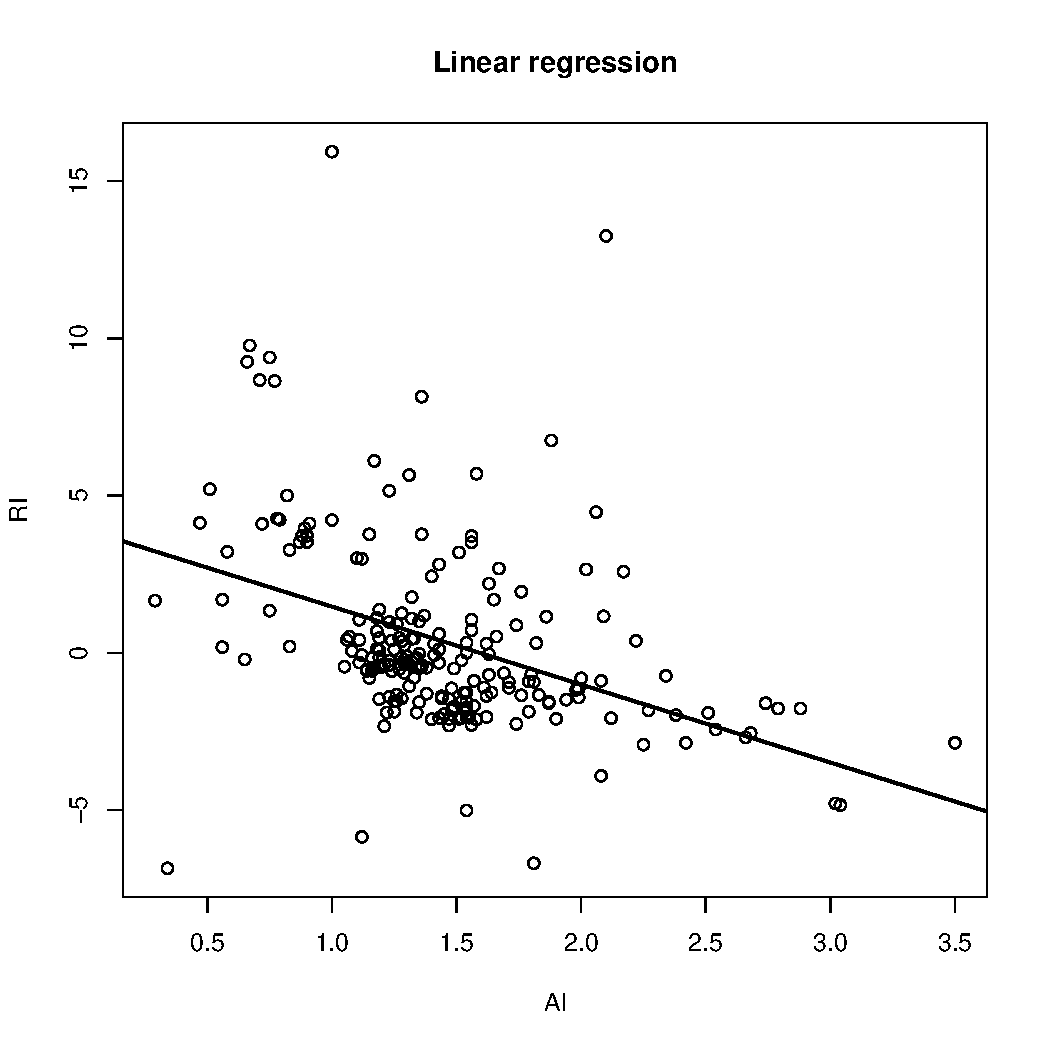
\includegraphics[page = 1, width = 0.8\textwidth]{glass.pdf}
    \end{center}
    \caption{
        A scatter plot of the given data. A linear regression line has been
        drawn to illustrate the general trend in the data, and to emphasize
        the need for nonparametric methods.
    }
    \label{fig:glass_linear}
    \end{figure}


    \section{Kernel regression}

    The Nadaraya-Watson estimator is of the form \[
        \widehat{m}(x) = \sum_{i = 1}^n \ell_i(x)\, y_i, \qquad
        \ell_i(x) = \frac{K((x - x_i) / h)}{\sum_{j = 1}^n K((x - x_j) / h)}.
    \] Here, we choose a Gaussian kernel $K(t) \propto e^{-t^2 / 2}$.

    Indeed, it can be shown that \[
        \widehat{m}(x) = \argmin_a \sum_{i = 1}^n w_i(x) (y_i - a)^2,
    \] where we choose weights $w_i(x) = K((x - x_i) / h)$.

    \begin{figure}[H]
    \begin{center}
        \includegraphics[page = 3, width = 0.8\textwidth]{glass.pdf}
    \end{center}
    \caption{
        Kernel regression, using the Gaussian kernel. Here, $h = 0.135$.
        We estimate $\widehat{\sigma}^2 \approx 6.53$.
    }
    \label{fig:glass_kernel}
    \end{figure}


    \section{Local linear regression}

    We estimate \[
        \widehat{m}(x) = \widehat{a}_0(x),
    \] where \[
        \widehat{\bm{a}}(x) = \argmin_{\bm{a}} \sum_{i = 1}^n
                w_i(x) (y_i - a_0 - a_1(x_i - x))^2.
    \] Note that by setting \[
        X = \begin{bmatrix}
            1 & x_1 - x \\
            1 & x_2 - x \\
            \vdots & \vdots \\
            1 & x_n  - x
        \end{bmatrix}, \qquad
        W = \operatorname{diag}(w_1(x), \dots, w_n(x)),
    \] we have \[
        \widehat{\bm{a}} = (X^\top W X)^- X^\top W \bm{y}.
    \]


    \begin{figure}[H]
    \begin{center}
        \includegraphics[page = 5, width = 0.8\textwidth]{glass.pdf}
    \end{center}
    \caption{
        Local linear regression, using the Gaussian kernel. Here, $h = 0.260$.
        We estimate $\widehat{\sigma}^2 \approx 6.41$.
    }
    \label{fig:glass_local_linear}
    \end{figure}



    \section{Cubic spline regression}

    Given a B-spline basis $\{B_i\}$ where all unique $x_i$'s are chosen as
    knots, we estimate \[
        \widehat{m}(x) = \sum_{j = 1}^{n + 4} \widehat{\beta}_j B_j(x).
    \] Here, $\widehat{\bm{\beta}}$ is chosen so as to minimize a penalized loss,
    i.e.\ \[
        \widehat{\bm{\beta}} = \argmin_{\bm{\beta}} \Vert \bm{y} -
        B\bm{\beta}\Vert^2 + \lambda\bm{\beta}^\top\Omega\bm{\beta},
    \] where \[
        B_{ij} = B_j(x_i), \qquad
        \Omega_{ij} = \int B_i'' B_j''.
    \] The parameter $\lambda > 0$ introduces a roughness penalty on
    $\widehat{m}$.

    Indeed, \[
        \widehat{\bm{\beta}} = (B^\top B + \lambda\Omega)^- B^\top \bm{y}.
    \]

    \begin{figure}[H]
    \begin{center}
        \includegraphics[page = 6, width = 0.8\textwidth]{glass.pdf}
    \end{center}
    \caption{
        Cubic spline regression, using all unique values of `Al' as knots.
        Here, the smoothing parameter $\lambda = 3.5\times 10^{-6}$.
        We estimate $\widehat{\sigma}^2 \approx 6.42$.
    }
    \label{fig:glass_spline}
    \end{figure}



    \section{Tuning parameters}

    In order to choose the parameters $h$ and $\lambda$, we use Ordinary
    Cross-Validation (OCV).

    Note that in all three cases, we have used \emph{linear smoothers}, in the
    sense that \[
        \widehat{m}(x) = L(x)\, \bm{y} = \sum_{i = 1}^n \ell_i(x) y_i.
    \] With this, the cross-validation score can be expressed as \[
        OCV = \frac{1}{n} \sum_{i = 1}^n \left(\frac{y_i - \widehat{m}(x_i)}{1
        - L_{ii}}\right)^2,
    \] where $L_{ii} = \ell_i(x_i)$. The parameter in question is chosen by
    minimizing the above.


    \section{Estimation of variance}

    With the setup of linear smoothers, a consistent estimator of the variance
    $\sigma^2$ (under certain conditions) is given by \[
        \widehat{\sigma}^2 = \frac{\sum_{i = 1}^n (y_i - \widehat{m}(x_i))^2}{n - 2\nu
        + \tilde{\nu}}, \qquad
        \nu = \trace(L), \qquad
        \tilde{\nu} = \trace(L^\top L).
    \] The quantity $\nu$ serves as an effective degrees of freedom.



    \section{Discussion}

    Visually, the kernel, local linear, and cubic spline regression curves
    look very similar. The kernel regression curve is slightly rougher than
    the rest.

    \begin{figure}[H]
    \begin{center}
        \includegraphics[page = 7, width = 0.8\textwidth]{glass.pdf}
    \end{center}
    \vspace{-1em}
    \caption{
       The linear, \textcolor{red}{kernel}, \textcolor{green}{local linear},
       and \textcolor{blue}{spline} regression curves.
    }
    \label{fig:glass_spline}
    \end{figure}

    On the other hand, the Ordinary Cross-Validation (OCV) score is minimum
    for the kernel regression ($6.85$), followed by the local linear
    regression ($7.17$) and finally the cubic spline regression ($8.74$).
    Thus, we choose the kernel regression method.



\end{document}
